% Copyright 2004 by Till Tantau <tantau@users.sourceforge.net>.
%
% In principle, this file can be redistributed and/or modified under
% the terms of the GNU Public License, version 2.
%
% However, this file is supposed to be a template to be modified
% for your own needs. For this reason, if you use this file as a
% template and not specifically distribute it as part of a another
% package/program, I grant the extra permission to freely copy and
% modify this file as you see fit and even to delete this copyright
% notice. 

\documentclass[aspectratio=169]{beamer}
%\documentclass{beamer}

\setbeamersize{text margin left=10mm, text margin right=10mm}

\defbeamertemplate{headline}{my header}{%
\vskip1pt%
\makebox[0pt][l]{\,\insertshortauthor}%
\hspace*{\fill}\insertshorttitle/\insertshortsubtitle\hspace*{\fill}%
\llap{\insertpagenumber/\insertpresentationendpage\,}
}
\setbeamertemplate{headline}[my header]

\usepackage{soul}
\usepackage{tkz-euclide}
\usetikzlibrary{calc}
\usepackage[]{algorithm2e}
\usepackage{changepage}
\usepackage{amssymb}
\usepackage{xcolor}
\usepackage{mathtools}
\usepackage{tcolorbox}
\usepackage{tikz}
\usetikzlibrary{arrows}
\usepackage{tikz-3dplot}
\usepackage{tkz-euclide}
\usepackage{circuitikz}
\usepackage{pgfplots}
\pgfplotsset{width=7cm,compat=1.8}

\usetikzlibrary{positioning}
% \usepackage[math]{cellspace}
% \cellspacetoplimit 4pt
% \cellspacebottomlimit 4pt
%\usetikzlibrary{arrows.meta}


%\setbeamertemplate{itemize items}{-}

%\usepackage{helvet}
\usefonttheme{professionalfonts} % using non standard fonts for beamer
%\usefonttheme{serif} % default family is serif
%\usepackage{fontspec}
%\setmainfont{Liberation Serif}

% There are many different themes available for Beamer. A comprehensive
% list with examples is given here:
% http://deic.uab.es/~iblanes/beamer_gallery/index_by_theme.html
% You can uncomment the themes below if you would like to use a different
% one:
%\usetheme{AnnArbor}
%\usetheme{Antibes}
%\usetheme{Bergen}
%\usetheme{Berkeley}
%\usetheme{Berlin}
%\usetheme{Boadilla}
%\usetheme{boxes}
%\usetheme{CambridgeUS}
%\usetheme{Copenhagen}
%\usetheme{Darmstadt}
%\usetheme{default}
%\usetheme{Frankfurt}
%\usetheme{Goettingen}
%\usetheme{Hannover}
%\usetheme{Ilmenau}
%\usetheme{JuanLesPins}
%\usetheme{Luebeck}
%\usetheme{Madrid}
%\usetheme{Malmoe}
%\usetheme{Marburg}
%\usetheme{Montpellier}
%\usetheme{PaloAlto}
%\usetheme{Pittsburgh}
%\usetheme{Rochester}
%\usetheme{Singapore}
%\usetheme{Szeged}
%\usetheme{Warsaw}

\def\mf{\ensuremath\mathbf}
\def\mb{\ensuremath\mathbb}
\def\lp{\ensuremath\left(}
\def\rp{\ensuremath\right)}
\def\lv{\ensuremath\left\lvert}
\def\rv{\ensuremath\right\rvert}
\def\lV{\ensuremath\left\lVert}
\def\rV{\ensuremath\right\rVert}
\def\lc{\ensuremath\left\{}
\def\rc{\ensuremath\right\}}
\def\bmx{\ensuremath\begin{bmatrix*}[r]}
\def\emx{\ensuremath\end{bmatrix*}}

\newcommand{\demoex}[2]{\onslide<#1->\begin{color}{black!60} #2 \end{color}}
\newcommand{\anim}[3]{\onslide<#1->{\begin{color}{#2!60} #3 \end{color}}}



\title{Linear Systems}

% A subtitle is optional and this may be deleted
\subtitle{Positive Definiteness and Matrix Norm}

\author{Sivakumar Balasubramanian}
% - Give the names in the same order as the appear in the paper.
% - Use the \inst{?} command only if the authors have different
%   affiliation.

\institute[Christian Medical College] % (optional, but mostly needed)
{
  \inst{}%
  Department of Bioengineering\\
  Christian Medical College, Bagayam\\
  Vellore 632002
}
% - Use the \inst command only if there are several affiliations.
% - Keep it simple, no one is interested in your street address.

\date{}
% - Either use conference name or its abbreviation.
% - Not really informative to the audience, more for people (including
%   yourself) who are reading the slides online

\subject{Lecture notes on linear systems}
% This is only inserted into the PDF information catalog. Can be left
% out. 

% If you have a file called "university-logo-filename.xxx", where xxx
% is a graphic format that can be processed by latex or pdflatex,
% resp., then you can add a logo as follows:

% \pgfdeclareimage[height=0.5cm]{university-logo}{university-logo-filename}
% \logo{\pgfuseimage{university-logo}}

% Delete this, if you do not want the table of contents to pop up at
% the beginning of each subsection:
\AtBeginSubsection[]
{
  \begin{frame}<beamer>{Outline}
    \tableofcontents[currentsection,currentsubsection]
  \end{frame}
}

% Let's get started
\begin{document}

\pgfplotsset{
  compat=1.8,
  colormap={whitered}{color(0cm)=(white); color(1cm)=(orange!75!red)}
}


\begin{frame}
  \titlepage
\end{frame}

\begin{frame}[t]{References}
\begin{itemize}
    \item G Strang, Linear Algebra: Chapters 6 and 7.
\end{itemize} 
\end{frame}


\begin{frame}[t]{Positive definite matrices}
\begin{itemize}
    \item We know that $\mf{x}^T\mf{x} > 0$ for all $\mf{x} \in \mb{R}^n$ and $\mf{x} \neq \mf{0}$.

    \item What can we say about $\mf{x}^T\mf{Ax}$, where $\mf{A} \in \mb{R}^{n \times n}$?
    \begin{itemize}
        \item Is it positive for all $\mf{x} \neq \mf{0}$?
        \anim{2}{blue}{
        E.g. $\mf{I}, \,\, \bmx3 & 0\\0 & 2\emx$
        }
        \item Can it be zero for some $\mf{x} \neq \mf{0}$? 
        \anim{3}{blue}{
        E.g. $\bmx1 & -1\\-1 & 1\emx$
        }
        \item Can it be negative some $\mf{x} \neq \mf{0}$? 
        \anim{4}{blue}{
        E.g. $\bmx-2 & 0\\0 & -1\emx, \bmx1 & -4\\-4 & 1\emx$
        }
    \end{itemize}

    \item Any matrix $\mf{A}$ for which $\mf{x}^T\mf{A}\mf{x} > 0$, for all $\mf{x} \neq \mf{0}$ is called a \textit{positive definite matrix}.

    \item Positive definite matrices are very useful and are commonly encountered in practice: optimization, mechanics (mass matrix, stiffness matrix), stability analysis, co-variance matrices etc. 
\end{itemize}
\demoex{5}{
    Are the following matrices positive definite: $\bmx 2 & -6\\2 & 1\emx, \bmx 5 & -1\\14 & 11\emx$
}
\end{frame}


\begin{frame}[t]{Positive Definite Matrix}
\vspace{-0.4cm}
\begin{small}
\begin{itemize}
    \item The idea of positive definiteness is intimately related to the problem of minimization of a function.

    \item Consider the following  function of a single variable $f\lp x\rp$. This function reaches a minimum at $x = 0$, when $\frac{df\lp x\rp}{dx} \big\rvert_{x=0} = 0$ and $\frac{d^2f\lp x\rp}{dx^2} \big\rvert_{x=0} > 0$. E.g.,
    $$f\lp x\rp = 3x^2 \rightarrow \frac{df\lp x\rp}{dx} \big\rvert_{x=0} = 0, \,\frac{d^2f\lp x\rp}{dx^2} \big\rvert_{x=0}  = 3 > 0$$

    \item What about $f\lp x_1, x_2 \rp = ax_1^2 + 2bx_1x_2 + cx_2^2$? We can extend the previous idea using partial derivatives.
    \[ \frac{\partial f\lp x_1, x_2 \rp}{\partial x_1} = 0, \,\, \frac{\partial f\lp x_1, x_2 \rp}{\partial x_2} = 0, \,\, \frac{\partial^2 f\lp x_1, x_2 \rp}{\partial x_1^2} > 0, \,\, \frac{\partial^2 f\lp x_1, x_2 \rp}{\partial x_2^2} > 0 \]
    Is this enough? $\frac{\partial^2f\lp x_1, x_2\rp}{\partial x_1 \partial x_2}$ must also be taken into account.
\end{itemize}

\demoex{2}{
    Are these functions positive for all $x_1, x_2$? 1) $x_1^2 + x_1x_2 + x_2^2$,\hspace{0.1cm}
}
\demoex{3}{
    2) $x_1^2 + 2x_1x_2 + x_2^2$,\hspace{0.1cm}
}
\demoex{4}{
    3) $x_1^2 + 3x_1x_2 + x_2^2$
}
\end{small}
\end{frame}


\begin{frame}[t]{Positive Definite Matrix}
\begin{itemize}
    \item We can rearrange $ax_1^2 + 2bx_1x_2 + cx_2^2$ in the following manner,
    \[ f\lp x_1, x_2 \rp = ax_1^2 + 2bx_1x_2 + cx_2^2 = a\lp x_1 + \frac{b}{a}x_2\rp^2 + \lp c - \frac{b^2}{a}\rp x_2^2 \]

    $f\lp\bullet\rp > 0, \forall x_1, x_2 \neq 0$ when,
    \[ a > 0\,\,\,\text{ and }\,\,\,c - \frac{b^2}{a} > 0 \implies ac > b^2 \]
    \[ \frac{\partial^2f\lp x_1, x_2 \rp}{\partial x_1^2} > 0\,\,\,\text{ and }\,\,\,\frac{\partial^2f\lp x_1, x_2 \rp}{\partial x_1^2} \frac{\partial^2f\lp x_1, x_2 \rp}{\partial x_2^2} > \lp\frac{\partial^2 f\lp x_1, x_2 \rp}{\partial x_1 \partial x_2}\rp^2 \]
\end{itemize}
\vspace{0.3cm}

\demoex{2}{
    Verfy this on the following functions: 1) $x_1^2 + x_1x_2 + x_2^2$,\hspace{0.1cm} 2) $x_1^2 + 2x_1x_2 + x_2^2$,\hspace{0.1cm} 3) $x_1^2 + 3x_1x_2 + x_2^2$
}
\end{frame}


\begin{frame}[t]{Positive Definite Matrix}
\vspace{-0.3cm}
$f\lp\bullet\rp$ can be expressed as $\mf{x}^T\mf{A}\mf{x}$, where $\mf{x} = \bmx x_1\\x_2 \emx$, and $\mf{A} = \bmx a & b\\b & c \emx$. $f\lp \mf{x}\rp > 0$ for all $\mf{x} \neq \mf{0}$, when $\mf{A}$ is positive definite.
\vspace{0.2cm}

$\mf{x}^T\mf{A}\mf{x}$ is called a \textit{quadratic form}. For a symmetric matrix $\mf{A}$,
\[ \mf{x}^T\mf{A}\mf{x} = \bmx
x_{1} & x_{2} & \ldots & x_{n}
\emx \bmx
a_{11} & a_{12} & \ldots & a_{1n}\\
a_{12} & a_{22} & \ldots & a_{2n}\\
\vdots & \vdots & \ddots & \vdots\\
a_{1n} & a_{2n} & \ldots & a_{nn}
\emx \bmx
x_{1} \\ x_{2} \\ \ldots \\ x_{n}
\emx = \sum_{i=1}^na_{ii}x_i^2 + 2\sum_{i=1}^n\sum_{j=1, j \neq i}^n a_{ij}x_ix_j \]

In general, $\mf{A} \in \mb{R}^{n \times n}$ is positive definite, if:
\begin{itemize}
    \item The eigenvalues of $\mf{A}$ are all positive.
    \item The pivots (without row exchange) are all positive.
\end{itemize}

\demoex{2}{
    Show that any $\mf{A}$ is positive definite if the symmetric matrix $\mf{A} + \mf{A}^T$ is positive definite. Note: \textit{This should explain why we have only been talking about symmetric matrices.}
}
\end{frame}


\begin{frame}[t]{Matrix Norm}
\begin{itemize}
    \item Since matrices also form vector spaces, we can talk about norms of matrices, which extent the idea of sizes and distances to spaces of matrices.

    \item If we think of matrices a set of $mn$ scalars, then we can use the same approach as vectors,
    \[ \lV \mf{A} \rV_F = \lp \sum_{i=1}^{m}\sum_{j=1}^{n}\lv a_{ij} \rv^2 \rp^\frac{1}{2} \]
    This is called the \textit{Frobinius norm}.    
\end{itemize}
\end{frame}


\begin{frame}[t]{Matrix Norm}
\begin{itemize}
    \item There are other norms defined for matrices that are very useful from the point of the view of linear transformation.

    \item These are called \textit{induced matrix norms}, that looks at how matrices map vectors from the range to domain spaces.

    \item Let $\mf{A} \in \mb{R}^{m \times n}: \mb{R}^n \to \mb{R}^m$, and $\mf{x} \in \mb{R}^n$, $\mf{y} \in \mb{R}^m$
    \[ \lV \mf{y} \rV = \lV \mf{A}\mf{x} \rV \leq C\lV\mf{x}\rV, \,\,\, \forall \mf{x} \in \mb{R}^n, \,\,\, C \geq 0 \]
    $C$ is the maximum factor by which $\mf{A}$ amplifies the vector $\mf{x}$.
    \item The induced norm of a matrix is defined as,
    \[  \lV \mf{A} \rV_p = \max_{\mf{x}} \frac{\lV \mf{A}\mf{x}\rV_p}{\lV \mf{x}\rV_p} = \max_{\lV\mf{x}\rV_p = 1} {\lV \mf{A}\mf{x}\rV_p} \]

\end{itemize}
\end{frame}


\begin{frame}[t]{Matrix Norm}
Consider a matrix $\mf{A} = \bmx 1 & 1 \\ 0 & 1\emx = \bmx \mf{a}_1 & \mf{a}_2\emx = \bmx \tilde{\mf{a}}_1^T \\ \tilde{\mf{a}}_2^T \emx$.\\

\begin{center}
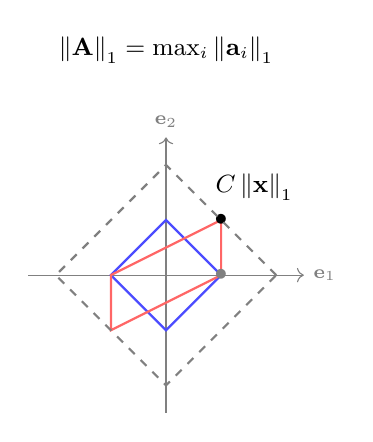
\begin{tikzpicture}[scale=0.7]
\draw[thin, gray, ->] (-2.5, 0) -- (2.5, 0) node[right] {\scriptsize{$\mf{e}_1$}};
\draw[thin, gray, ->] (0, -2.5) -- (0, 2.5) node[above] {\scriptsize{$\mf{e}_2$}};

\draw[thick, blue!70!, -] (1, 0) -- (0, 1) -- (-1, 0) -- (0, -1) -- (1, 0);
\draw[thick, red!60!, -] (1, 0) -- (1, 1) -- (-1, 0) -- (-1, -1) -- (1, 0);
\node[gray] at (1, 0) {\small{$\bullet$}};
\node[black] at (1, 1) {\small{$\bullet$}};
\node[below, black] at (0.0, 4.5) {\small{$\lV\mf{A}\rV_1 = \max_i \lV \mf{a}_i\rV_1$}};
\draw[thick, gray, dashed] (2, 0) -- (0, 2) -- (-2, 0) -- (0, -2) -- (2, 0);
\node[black] at (1.6, 1.6) {\small{$C\lV\mf{x}\rV_1$}};
\end{tikzpicture} \hspace{0.1cm}
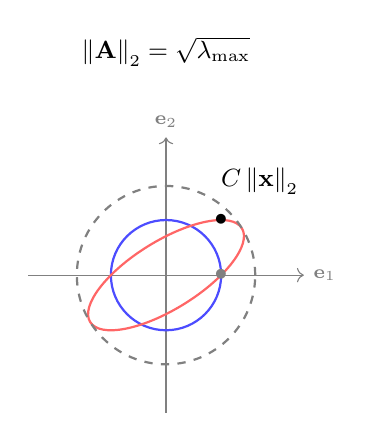
\begin{tikzpicture}[scale=0.7]
\draw[thin, gray, ->] (-2.5, 0) -- (2.5, 0) node[right] {\scriptsize{$\mf{e}_1$}};
\draw[thin, gray, ->] (0, -2.5) -- (0, 2.5) node[above] {\scriptsize{$\mf{e}_2$}};
\draw[thick, blue!70!] (0,0) circle (1);
\draw[thick, red!60!, rotate=31.72] (0,0) ellipse (1.61803 and 0.61803);
\node[gray] at (1, 0) {\small{$\bullet$}};
\node[black] at (1, 1) {\small{$\bullet$}};
\node[below, black] at (0.0, 4.5) {\small{$\lV\mf{A}\rV_2 = \sqrt{\lambda_{\max}}$}};
\draw[thick, gray, dashed] (0,0) circle (1.61803);
\node[black] at (1.7, 1.7) {\small{$C\lV\mf{x}\rV_2$}};
\end{tikzpicture} \hspace{0.1cm}
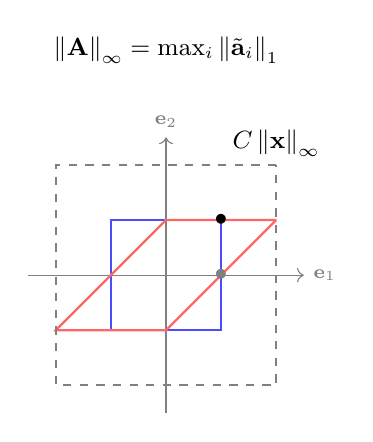
\begin{tikzpicture}[scale=0.7]
\draw[thin, gray, ->] (-2.5, 0) -- (2.5, 0) node[right] {\scriptsize{$\mf{e}_1$}};
\draw[thin, gray, ->] (0, -2.5) -- (0, 2.5) node[above] {\scriptsize{$\mf{e}_2$}};
\draw[thick, blue!70!, -] (1, 1) -- (-1, 1) -- (-1, -1) -- (1, -1) -- (1, 1);
\draw[thick, red!60!, -] (2, 1) -- (0, 1) -- (-2, -1) -- (0, -1) -- (2, 1);
\node[gray] at (1, 0) {\small{$\bullet$}};
\node[black] at (1, 1) {\small{$\bullet$}};
\node[below, black] at (0.0, 4.5) {\small{$\lV\mf{A}\rV_\infty = \max_i \lV \tilde{\mf{a}}_i\rV_1$}};
\draw[thick, gray, dashed] (2, 2) -- (-2, 2) -- (-2, -2) -- (2, -2) -- (2, 2);
\node[black] at (2.0, 2.4) {\small{$C\lV\mf{x}\rV_\infty$}};
\end{tikzpicture}
\end{center}
\end{frame}


 \end{document}